\documentclass[a4paper]{article}

\input{style/ch_xelatex.tex}
\input{style/scala.tex}

%代码段设置
\lstset{numbers=left,
basicstyle=\tiny,
numberstyle=\tiny,
keywordstyle=\color{blue!70},
commentstyle=\color{red!50!green!50!blue!50},
frame=single, rulesepcolor=\color{red!20!green!20!blue!20},
escapeinside=``
}

\graphicspath{ {images/} }
\usepackage{ctex}
\usepackage{graphicx}
\usepackage{color,framed}%文本框
\usepackage{listings}
\usepackage{caption}
\usepackage{amssymb}
\usepackage{enumerate}
\usepackage{xcolor}
\usepackage{bm}
\usepackage{lastpage}%获得总页数
\usepackage{fancyhdr}
\usepackage{tabularx}
\usepackage{geometry}
\usepackage{minted}
\usepackage{graphics}
\usepackage{subfigure}
\usepackage{float}
\usepackage{pdfpages}
\usepackage{pgfplots}
\pgfplotsset{width=10cm,compat=1.9}
\usepackage{multirow}
\usepackage{footnote}
\usepackage{booktabs}

%-----------------------伪代码------------------
\usepackage{algorithm}
\usepackage{algorithmicx}
\usepackage{algpseudocode}
\floatname{algorithm}{Algorithm}
\renewcommand{\algorithmicrequire}{\textbf{Input:}}
\renewcommand{\algorithmicensure}{\textbf{Output:}}
\usepackage{lipsum}
\makeatletter
\newenvironment{breakablealgorithm}
  {% \begin{breakablealgorithm}
  \begin{center}
     \refstepcounter{algorithm}% New algorithm
     \hrule height.8pt depth0pt \kern2pt% \@fs@pre for \@fs@ruled
     \renewcommand{\caption}[2][\relax]{% Make a new \caption
      {\raggedright\textbf{\ALG@name~\thealgorithm} ##2\par}%
      \ifx\relax##1\relax % #1 is \relax
         \addcontentsline{loa}{algorithm}{\protect\numberline{\thealgorithm}##2}%
      \else % #1 is not \relax
         \addcontentsline{loa}{algorithm}{\protect\numberline{\thealgorithm}##1}%
      \fi
      \kern2pt\hrule\kern2pt
     }
  }{% \end{breakablealgorithm}
     \kern2pt\hrule\relax% \@fs@post for \@fs@ruled
  \end{center}
  }
\makeatother
%------------------------代码-------------------
\usepackage{xcolor}
\usepackage{listings}
\lstset{
breaklines,%自动换行
basicstyle=\small,
escapeinside=``,
keywordstyle=\color{ blue!70} \bfseries,
commentstyle=\color{red!50!green!50!blue!50},%
stringstyle=\ttfamily,%
extendedchars=false,%
linewidth=\textwidth,%
numbers=left,%
numberstyle=\tiny \color{blue!50},%
frame=trbl%
rulesepcolor= \color{ red!20!green!20!blue!20}
}

%-------------------------页面边距--------------
\geometry{a4paper,left=2.3cm,right=2.3cm,top=2.7cm,bottom=2.7cm}
%-------------------------页眉页脚--------------
\usepackage{fancyhdr}
\pagestyle{fancy}
\lhead{\kaishu \leftmark}
% \chead{}
\rhead{\kaishu 深度学习进阶课 实验报告}%加粗\bfseries
\lfoot{}
\cfoot{\thepage}
\rfoot{}
\renewcommand{\headrulewidth}{0.1pt}
\renewcommand{\footrulewidth}{0pt}%去掉横线
\newcommand{\HRule}{\rule{\linewidth}{0.5mm}}%标题横线
\newcommand{\HRulegrossa}{\rule{\linewidth}{1.2mm}}
\setlength{\textfloatsep}{10mm}%设置图片的前后间距

%----------------------实验结果数字（评测后统一填这里）----------------------
\newcommand{\bestEpoch}{20}      % dev 上最优 epoch
\newcommand{\devWER}{12.29}      % 最优 dev WER (%)
\newcommand{\testWER}{10.84}     % test WER (%)
\newcommand{\testSub}{1593}      % test 替换错误数
\newcommand{\testDel}{149}       % test 删除错误数
\newcommand{\testIns}{175}       % test 插入错误数
\newcommand{\testN}{17682}       % test 参考拼音总数
\newcommand{\testLoss}{0.398}    % test CTC loss

%--------------------文档内容--------------------

\begin{document}
\renewcommand{\contentsname}{目\ 录}
\renewcommand{\appendixname}{附录}
\renewcommand{\appendixpagename}{附录}
\renewcommand{\refname}{参考文献}
\renewcommand{\figurename}{图}
\renewcommand{\tablename}{表}
\renewcommand{\today}{\number\year 年 \number\month 月 \number\day 日}

%-------------------------封面----------------
\begin{titlepage}
    \begin{center}
    \includegraphics[width=0.8\textwidth]{NKU.png}\\[1cm]
    \vspace{20mm}
		\textbf{\huge\textbf{\kaishu{计算机学院}}}\\[0.5cm]
		\textbf{\huge{\kaishu{语音信息处理实验报告}}}\\[2.3cm]
		\textbf{\Huge\textbf{\kaishu{基于 AI Coding 的语音识别：\\[0.3cm]Transformer Encoder + CTC 拼音识别}}}

		\vspace{\fill}

    \centering
    \textsc{\LARGE \kaishu{姓名\ :\ 申健强}}\\[0.5cm]
    \textsc{\LARGE \kaishu{学号\ :\ 2313119}}\\[0.5cm]
    \textsc{\LARGE \kaishu{专业\ :\ 计算机科学与技术}}\\[0.5cm]

    \vfill
    {\Large \today}
    \end{center}
\end{titlepage}

\renewcommand {\thefigure}{\thesection{}.\arabic{figure}}%图片按章标号
\renewcommand{\figurename}{图}
\renewcommand{\contentsname}{目录}
\cfoot{\thepage\ of \pageref{LastPage}}%当前页 of 总页数

% 生成目录
\clearpage
\tableofcontents
\newpage

%--------------------------正文--------------------------------
\section{实验目的与内容}
本实验以「基于 AI Coding 的语音识别」为主题，借助大模型（豆包）与 Vibe Coding 的方式，实现一个
以 \textbf{Transformer Encoder + CTC} 为框架的中文语音识别系统。识别目标是不带声调的\textbf{拼音}序列，
数据集为标贝中文语音库（BZNSYP，约 12 小时、共 10000 条），已划分为 8000 条训练、1000 条验证、1000 条测试。
助教已用豆包实现好数据处理与模型两部分代码，需要自行（借助 AI）补全的是\textbf{训练、推理解码与 WER 评测}三段，
最终目标是在测试集上把词错误率 WER 压到 30\% 以内。实验内容包括：

\begin{enumerate}
  \item 走通完整 ASR 流程：Fbank 特征提取、拼音词表构建、变长数据对齐、CTC 训练、贪心解码、WER 评测。
  \item 理解 CTC 如何解决语音帧序列（长度 $T$）与拼音序列（长度 $L$，$T\gg L$）之间的对齐问题。
  \item 完成训练/推理/评测代码，训练模型并在测试集上报告 WER，达标线为 WER $<30\%$。
  \item 进阶任务：与 AI 讨论并对模型做出改进，分析改进有效或无效的原因。
  \item 结合本次开发体验，回答关于使用 AI 编程的若干开放性问题。
\end{enumerate}

实验环境为 \texttt{speechbrain} conda 环境（Python 3.10，torch 2.1.2+cu118，torchaudio 2.1.2+cu118），
训练运行于本地 GPU（NVIDIA RTX 4060 Laptop）。虽然 PPT 指出 CPU 即可完成，但本地 GPU 免费且更快，
单个 epoch 约 70 秒。

\section{实验原理}
\subsection{语音识别与 CTC}
语音识别（ASR）把一段语音转录为文本，本质是把不定长的语音帧序列映射为不定长的符号（这里是拼音）序列。
难点在于二者\textbf{没有显式的对齐关系}：一段语音提取特征后有 $T$ 帧（可能几百帧），对应的拼音只有 $L$ 个
（$T\gg L$），而且不知道哪几帧对应哪个拼音。

CTC（Connectionist Temporal Classification）\cite{ctc} 通过引入一个特殊的\textbf{空白符 blank} 来解决对齐。
模型对每一帧都输出一个在词表（含 blank）上的分布，得到一条长度为 $T$ 的帧级路径 $\pi$；再用一个多对一的
压缩函数 $\mathcal{B}$ 把路径映射回拼音序列：先\textbf{合并相邻相同符号}，再\textbf{删除所有 blank}。例如
\begin{equation}
  \mathcal{B}(\;[\varnothing,\text{ka},\text{ka},\varnothing,\text{e},\text{e},\varnothing]\;)=[\text{ka},\text{e}],
\end{equation}
其中 $\varnothing$ 表示 blank。blank 的关键作用是区分「同一个拼音持续多帧」与「两个相同拼音相连」：
只有输出 blank 或新符号时才前进到下一个符号，因此想输出两个连续相同的拼音必须靠中间的 blank 隔开。

CTC 的对齐可以用图~\ref{fig:lattice} 的网格（trellis）直观理解：横轴是输入的 $T$ 个语音帧 $x_1,\dots,x_T$，
纵轴是目标序列插入 blank 后的状态（$\varnothing,a,\varnothing,b,\varnothing$）。一条从左上到右下、
每步只能向右或右下走的路径就是一种对齐方式，图中标出的多条深色路径都会被 $\mathcal{B}$ 压缩成同一个结果
$[a,b]$。节点 $(s,t)$ 上的 $\alpha_{s,t}$ 是「前 $t$ 帧对齐到前 $s$ 个状态」的所有路径概率之和，
可用前向-后向动态规划高效递推。

\begin{figure}[H]
    \centering
    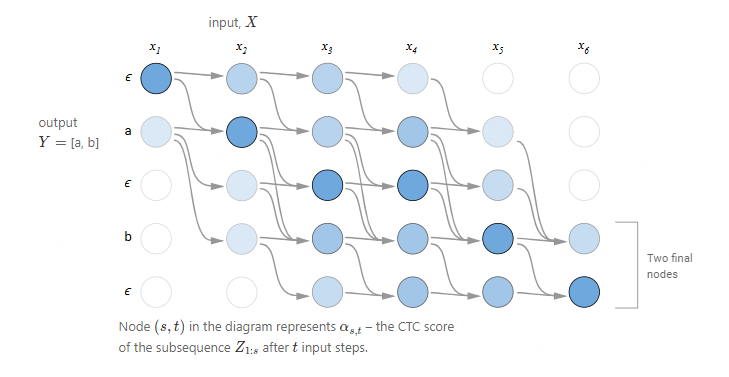
\includegraphics[width=0.72\textwidth]{ppt_ctc_lattice.png}
    \caption{CTC 对齐网格（引自课程课件）。横轴为输入帧，纵轴为插入 blank 后的目标状态；
    从左上到右下的每条路径都是一种合法对齐，均可压缩成 $Y=[a,b]$，节点值 $\alpha_{s,t}$ 为 CTC 前向得分。}
    \label{fig:lattice}
\end{figure}

\textbf{训练}时，一个正确拼音序列 $\mathbf{y}$ 对应许多条能被 $\mathcal{B}$ 压缩成它的路径，CTC 用前向-后向
（动态规划）把所有合法路径的概率求和，最小化其负对数似然：
\begin{equation}
  \mathcal{L}_{\text{CTC}}=-\log\!\!\sum_{\pi\in\mathcal{B}^{-1}(\mathbf{y})} p(\pi\mid \mathbf{X})
  =-\log\!\!\sum_{\pi\in\mathcal{B}^{-1}(\mathbf{y})}\prod_{t=1}^{T} p(\pi_t\mid \mathbf{X}).
\end{equation}
\textbf{推理}时采用贪心解码：对每帧取概率最大的符号得到路径，再用同一个 $\mathcal{B}$ 压缩（合并重复 + 去 blank）
得到最终拼音序列。

\subsection{Transformer Encoder + CTC 架构}
整个系统的数据流为：
\begin{center}
音频 $\rightarrow$ Fbank(80维) $\rightarrow$ 卷积下采样($4\times$) $\rightarrow$ Transformer Encoder
$\rightarrow$ CTC 线性头(每帧输出词表分布) $\rightarrow$ 贪心解码 $\rightarrow$ 拼音。
\end{center}
其中 Transformer Encoder 由自注意力和前馈网络堆叠而成，负责为每一帧建模上下文；由于 CTC 依赖时序顺序，
必须为其提供\textbf{位置编码}。CTC 头对每帧独立地把 encoder 输出映射到词表维度并做 log-softmax。

\subsection{评测指标 WER}
以拼音为单位，用词错误率 WER 衡量识别质量。把预测序列对齐到参考序列（最小编辑距离），统计三类错误：
替换 $S$、删除 $D$、插入 $I$，则
\begin{equation}
  \text{WER}=\frac{S+D+I}{N},
\end{equation}
$N$ 为参考序列中的拼音总数（图~\ref{fig:wer}）。WER 越低越好；若预测为空串，则全部计为删除错误，WER 为 $100\%$。

\begin{figure}[H]
    \centering
    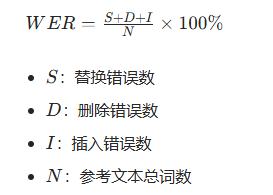
\includegraphics[width=0.5\textwidth]{ppt_wer.png}
    \caption{WER 的定义与三类错误 $S/D/I$（引自课程课件）。}
    \label{fig:wer}
\end{figure}

\section{数据与预处理}
预处理部分（豆包已实现）需要同时处理语音和拼音两个模态，整体数据流见图~\ref{fig:pipeline}：
从原始 WAV、\texttt{wav.scp} 与拼音文本出发，依次经词表构建、特征提取、数据集封装、加载器封装，
最终喂给 ASR 模型训练与推理。各模块的作用见表~\ref{tab:pre}。

\begin{figure}[H]
    \centering
    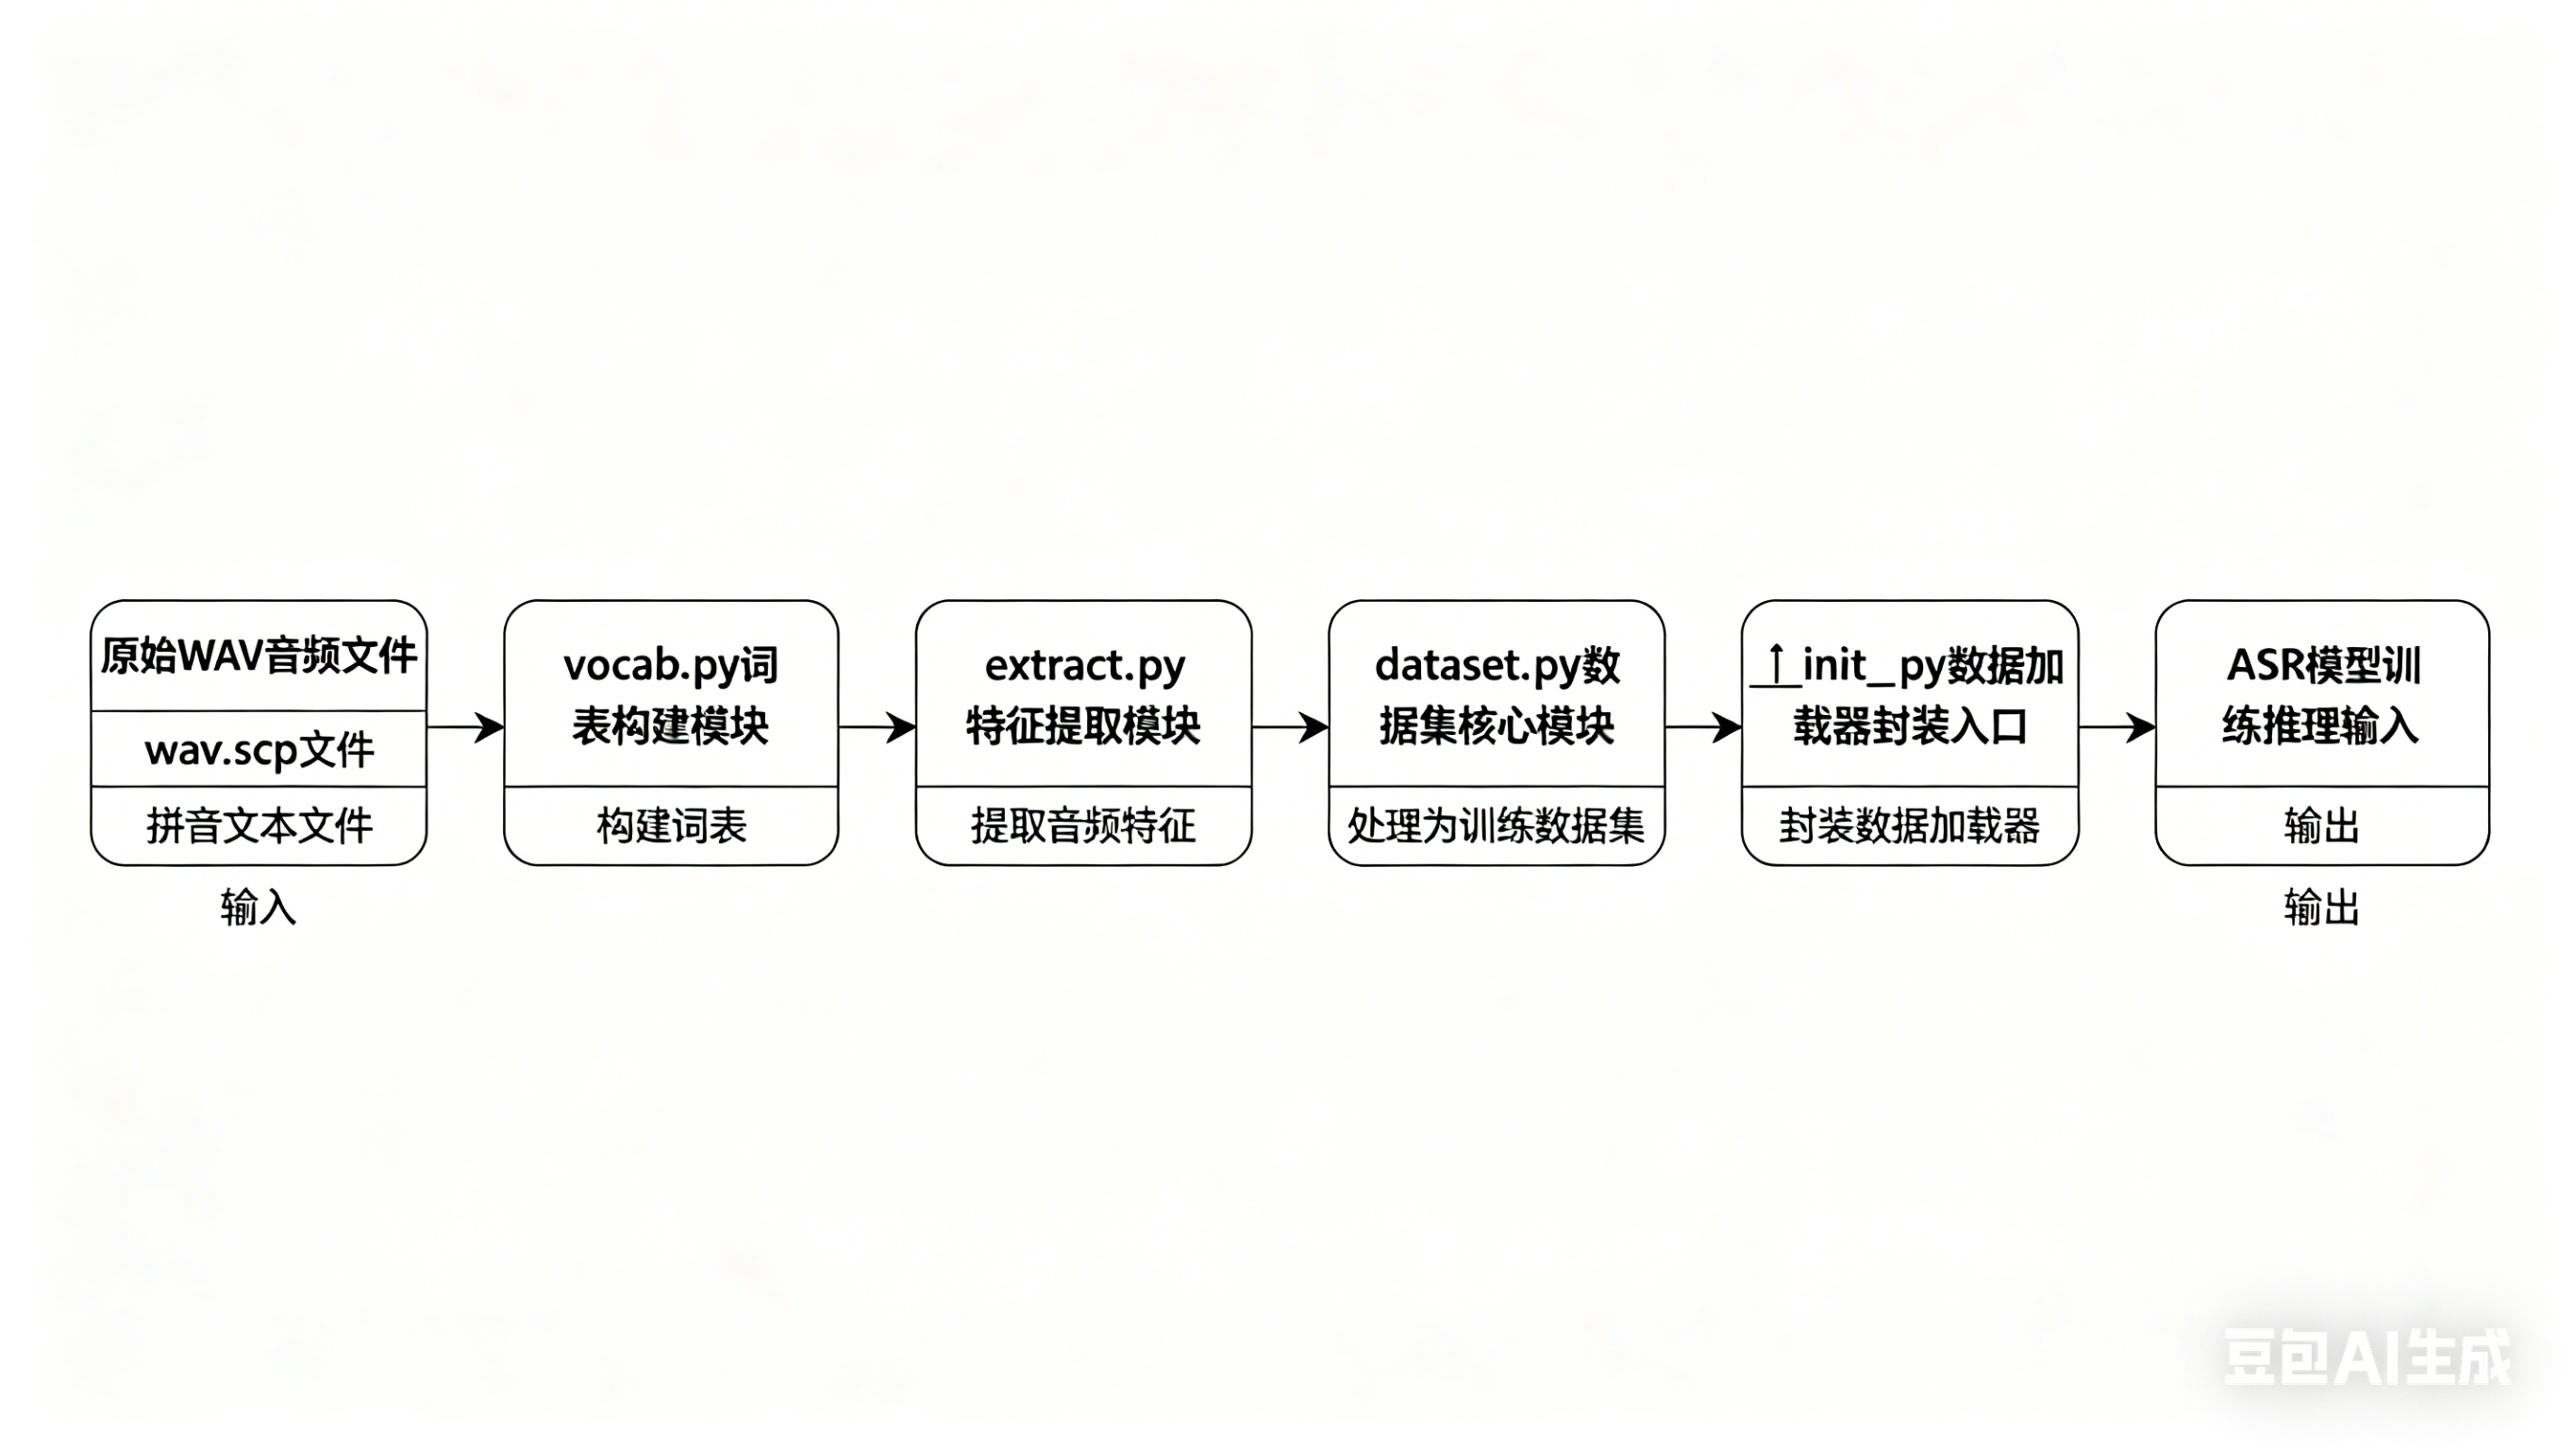
\includegraphics[width=\textwidth]{ppt_pipeline.png}
    \caption{数据处理流水线（引自课程课件）：原始音频与标注 $\rightarrow$ 词表/特征/数据集 $\rightarrow$ 加载器 $\rightarrow$ ASR 模型。}
    \label{fig:pipeline}
\end{figure}

\begin{table}[H]
  \centering
  \begin{tabularx}{\textwidth}{l X}
  \toprule
  模块 & 作用 \\
  \midrule
  \texttt{extract\_fbank} & 加载音频，重采样到 16k、转单声道，用 Kaldi 兼容接口提取 80 维 Fbank，并做倒谱均值归一化(CMN) \\
  \texttt{Vocab} & 从训练集拼音统计词表，索引 0 固定为 blank，实现拼音$\leftrightarrow$索引互转及 CTC 解码 \\
  \texttt{ASRDataset} & 读取 \texttt{wav.scp} 与 \texttt{pinyin}，取二者交集，返回 (Fbank, 标签索引) \\
  \texttt{collate\_fn} & 对一个 batch 内变长的特征与标签做 padding 对齐，并记录原始长度供 CTC 使用 \\
  \bottomrule
  \end{tabularx}
  \caption{数据预处理的主要模块。}
  \label{tab:pre}
\end{table}

其中 \texttt{collate\_fn} 是重点：音频和拼音都是变长的，同一个 batch 必须长度一致才能堆成张量。它用
\texttt{pad\_sequence} 把特征 padding 到本 batch 最长帧数、把标签 padding 到最长拼音数，同时返回两者的
\textbf{原始长度}（\texttt{feature\_lengths}、\texttt{label\_lengths}）。这两个长度是 CTC 损失的必需输入：
CTC 靠它们只在有效范围内计算，从而正确忽略 padding。词表大小为 407（406 个拼音 + 1 个 blank）。

\section{模型：Transformer Encoder + CTC}
模型 \texttt{ASRTransformerCTC}（豆包实现，本实验做了关键修正，见第~\ref{sec:debug} 节）由四部分组成，
配置见表~\ref{tab:model}。

\begin{table}[H]
  \centering
  \begin{tabularx}{\textwidth}{l X}
  \toprule
  组件 & 说明 \\
  \midrule
  \texttt{ConvSubsampling} & 两层 stride=2 的 2D 卷积，把时间维压缩 $4\times$，同时把 80 维特征投影到 $d_{\text{model}}$。降低算力并缩短序列 \\
  \texttt{PositionalEncoding} & 正弦位置编码，为注意力提供时序信息 \\
  \texttt{TransformerEncoder} & $6$ 层，$d_{\text{model}}{=}256$、$4$ 头、前馈 $1024$、dropout $0.1$，Pre-LN \\
  \texttt{ctc\_head} & 线性层 $256\rightarrow 407$，接 log-softmax，输出每帧词表分布 \\
  \bottomrule
  \end{tabularx}
  \caption{模型组件与超参数（约 6.45M 参数）。}
  \label{tab:model}
\end{table}

值得强调的三个实现细节，都是 CTC 系统里「不报错但会算错」的高发点，本实验实现时逐一对齐：
\begin{enumerate}
  \item \textbf{blank 三处一致}：词表里 blank 固定为 0、\texttt{nn.CTCLoss(blank=0)}、解码去 blank 都用 0，
        任一处不一致都会导致训练不收敛却不报错。
  \item \textbf{张量形状 $[T,B,V]$}：PyTorch 的 CTCLoss 要求 log-probs 时间维在前，模型前向最后
        转成 $[\,$SeqLen, Batch, Vocab$\,]$ 返回。
  \item \textbf{下采样后的长度}：卷积把帧数压了 $4\times$，传给 CTC 的 \texttt{input\_lengths} 必须是
        \emph{下采样后}的长度（模型返回的 \texttt{output\_lengths}），而非原始帧数，否则会越界导致 loss 变
        \texttt{nan}。本实验诊断确认全部样本满足「下采样长度 $\ge$ 目标长度」（中位数比值约 6.8），
        并在 CTCLoss 中开启 \texttt{zero\_infinity=True} 作为额外保险。
\end{enumerate}

\section{训练、推理与评测的实现}
\subsection{训练脚本}
训练脚本 \texttt{train.py} 的关键设置：优化器 Adam（$\text{lr}=10^{-3}$，权重衰减 $10^{-6}$）；学习率采用
\textbf{线性 warmup（400 步）+ 余弦退火}；梯度裁剪范数 5.0；损失为 \texttt{nn.CTCLoss(blank=0, zero\_infinity=True)}；
batch size 16，训练 20 个 epoch。每个 epoch 结束在验证集上计算 CTC loss 与 WER，保存该 epoch 权重，
并按 \textbf{dev WER 最优}原则另存 \texttt{best.pt}。用 dev 挑最优 epoch、再固定评测 test，避免用测试集调参。
（助教参考配置为更小的 $d_{\text{model}}{=}128$、$\text{lr}=10^{-4}$、batch 8、10 epoch；本实验因改用 Pre-LN
而能用高 10 倍的 $\text{lr}=10^{-3}$ 更快收敛，并把模型适当加大到 $d_{\text{model}}{=}256$。）

\subsection{推理解码与 WER}
推理采用贪心 CTC 解码：对模型输出 $[T,B,V]$ 在词表维取 argmax 得到帧级路径，按 \texttt{output\_lengths}
截断有效长度，再调用词表的解码函数「合并相邻重复 + 去 blank」得到拼音串。WER 由自己实现的编辑距离
（带回溯）统计语料级的 $S/D/I/N$ 后按式 (3) 计算。

\section{关键问题的定位与修复：从「全 blank 塌缩」到 Pre-LN}
\label{sec:debug}
这是本次实验最有价值的部分，完整体现了「AI 生成的代码出错 $\rightarrow$ 定位根因 $\rightarrow$ 修正」的过程。

\subsection{现象}
按豆包给出的模型直接训练，\textbf{10 个 epoch 全程 WER $=100\%$}：贪心解码输出\textbf{空串}，全部记为删除错误
（$S{=}0,I{=}0$）。train loss 在第 2 个 epoch 后就卡在 $\approx 5.64$ 几乎不动（词表 407 的均匀分布约为 $6.0$，
说明模型几乎什么都没学到）。这是 CTC 典型的\textbf{全 blank 塌缩}：模型陷入「每帧都预测 blank」这个平凡解的
局部极小，且没能自己逃出来。

\subsection{定位过程}
按「CTC 系统按环节排查」的思路逐一排除：
\begin{enumerate}
  \item \textbf{数据/长度}：写诊断脚本检查特征尺度（mean$\approx 0$，std$\approx 3.8$，正常）与下采样长度，
        确认 $0\%$ 样本出现 \texttt{input\_len < target\_len}，排除 \texttt{zero\_infinity} 静默丢样本导致的梯度饥饿。
  \item \textbf{学习率（双向验证）}：先怀疑 LR 太低跳不出盆地，把峰值 LR 提到 $2\times10^{-3}$——\textbf{仍然塌缩}；
        反过来用助教参考配置的 $\text{lr}=10^{-4}$（低 10 倍）重训，\textbf{Post-LN 竟然能正常收敛}
        （6 个 epoch 内 dev WER 从 $100\%$ 降到 $40.8\%$）。这说明问题恰恰\textbf{与学习率强相关、但方向相反}：
        Post-LN 在较高 LR 下不稳定、直接塌缩，只有很低的 LR 才能训、但收敛很慢。
  \item \textbf{归一化位置}：train loss 在高 LR 下完全平坦（而非缓慢下降）指向\textbf{梯度不稳、不流动}。
        豆包实现的是 \textbf{Post-LN}（后置 LayerNorm）Transformer，这类结构从零训练对学习率敏感、需极小心地调参；
        据此把它换成 \textbf{Pre-LN}，在同样较高的 $\text{lr}=10^{-3}$ 下即稳健收敛，从而锁定根因。
\end{enumerate}

\subsection{修复}
把 Transformer 改为 \textbf{Pre-LN（\texttt{norm\_first=True}）}，并按 Pre-LN 的标准做法在编码器堆栈末尾补一个
\textbf{最终 LayerNorm}（PyTorch 默认不加，会使残差流不归一化就进 CTC 头）。改动仅数行，效果立竿见影：
在较高的 $\text{lr}=10^{-3}$ 下，4 个 epoch 内 dev WER 就从 $100\%$ 依次降到
$37.5\%\rightarrow 29.4\%\rightarrow 26.9\%\rightarrow 23.3\%$，比 Post-LN 只能用低 LR 慢慢训要快得多。
三种设置的对比见表~\ref{tab:ablation} 与图~\ref{fig:ablation}。

\begin{table}[H]
  \centering
  \begin{tabular}{llccccl}
  \toprule
  设置 & 学习率 & ep1 & ep2 & ep3 & ep4 & 结果 \\
  \midrule
  Post-LN（原始） & $10^{-3}$ & 100\% & 100\% & 100\% & 100\% & 塌缩 \\
  Post-LN（原始） & $10^{-4}$ & 100\% & 72.3\% & 53.4\% & 45.4\% & 慢但能训 \\
  Pre-LN（修复后） & $10^{-3}$ & 37.5\% & 29.4\% & 26.9\% & 23.3\% & 又快又稳 \\
  \bottomrule
  \end{tabular}
  \caption{三种设置前 4 个 epoch 的 dev WER。Post-LN 对学习率敏感（高 LR 塌缩、低 LR 慢），Pre-LN 在高 LR 下稳健且最快。}
  \label{tab:ablation}
\end{table}

\begin{figure}[H]
    \centering
    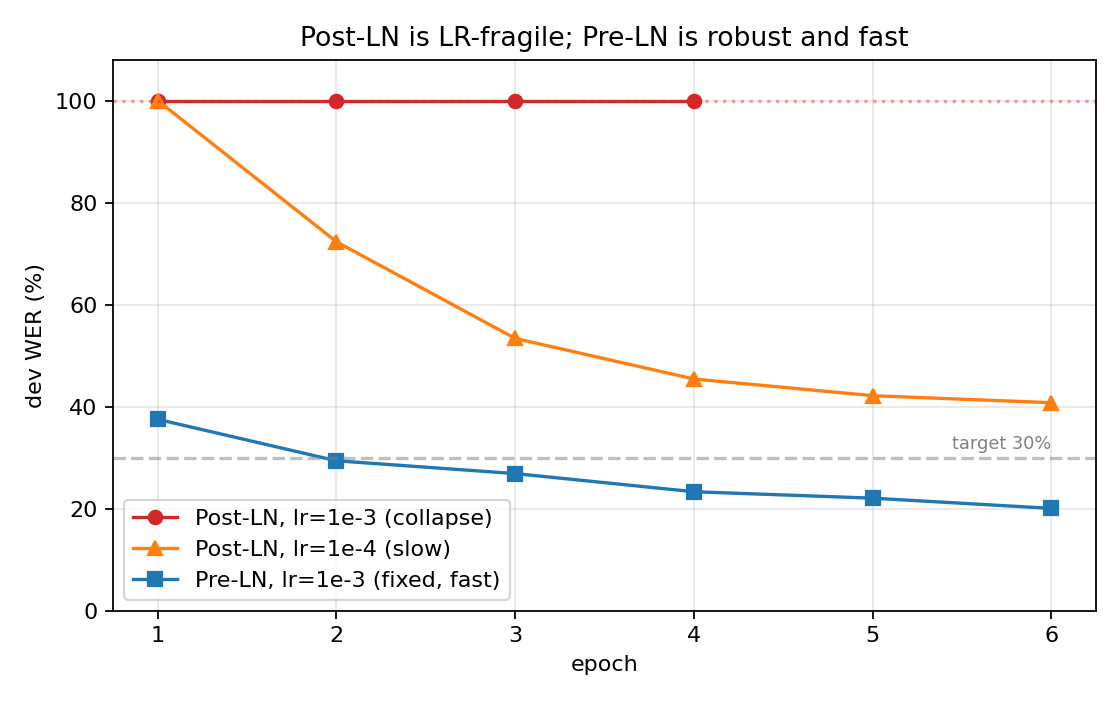
\includegraphics[width=0.72\textwidth]{res_prenorm_ablation.png}
    \caption{三种设置的 dev WER 对比：Post-LN 在 $\text{lr}=10^{-3}$ 塌缩、在 $\text{lr}=10^{-4}$ 缓慢收敛，
    Pre-LN 在 $\text{lr}=10^{-3}$ 又快又稳（2 个 epoch 即越过 $30\%$ 目标线）。}
    \label{fig:ablation}
\end{figure}

\textbf{原因分析}：Post-LN 把 LayerNorm 放在残差相加\emph{之后}，深层堆叠时反向传播的梯度要穿过多层未归一化的
乘法链，对学习率非常敏感，常需要很小心的 warmup 和很小的 LR 才能启动；而 Pre-LN 把 LayerNorm 放在子层\emph{之前}，
残差是一条「干净」的恒等通路，梯度可以直接回流，训练稳定性大幅提升。这也解释了为什么助教必须用很低的
$\text{lr}=10^{-4}$——那是让 Post-LN 勉强稳定的代价；而 Pre-LN 从结构上解决了梯度回流，因此能直接用更高的
$\text{lr}=10^{-3}$ 又快又稳地训练，让模型顺利跳出全 blank 平凡解。这也印证了 PPT 最后一页的提示——
豆包生成的代码可能有错误，需要使用者具备判断力去定位和修正。

\section{实验结果}
以修复后的 Pre-LN 模型，采用上述训练配置训练 20 个 epoch。训练/验证 loss 与 dev WER 随 epoch 的变化见
图~\ref{fig:curve}：loss 稳定下降，dev WER 在第 \bestEpoch{} 个 epoch 取得最优 \devWER\%。

\begin{figure}[H]
    \centering
    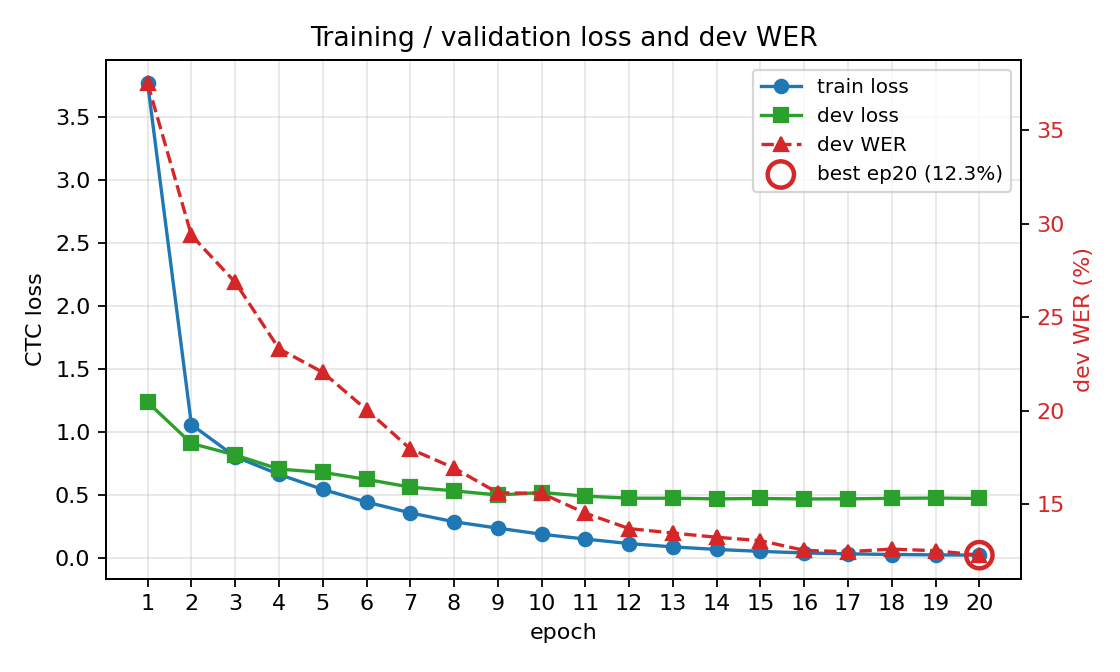
\includegraphics[width=0.8\textwidth]{res_train_curve.png}
    \caption{训练/验证 CTC loss（左轴）与 dev WER（右轴）随 epoch 的变化，圈标处为 dev 最优 epoch。}
    \label{fig:curve}
\end{figure}

固定 dev 最优的 \texttt{best.pt}，在测试集上评测，结果见表~\ref{tab:result}。\textbf{测试集 WER 为 \testWER\%，
达到并优于 $30\%$ 的目标}。错误组成（图~\ref{fig:break}）以替换错误为主，说明模型基本能定位到发音位置，
主要是把某些拼音混淆成了发音相近的拼音，符合朗读语音上 CTC 拼音识别的预期。

\begin{table}[H]
  \centering
  \begin{tabular}{lccccc}
  \toprule
  数据集 & WER & 替换 $S$ & 删除 $D$ & 插入 $I$ & 参考拼音数 $N$ \\
  \midrule
  dev（第 \bestEpoch{} epoch） & \devWER\% & 1781 & 210 & 129 & 17252 \\
  test & \testWER\% & \testSub{} & \testDel{} & \testIns{} & \testN{} \\
  \bottomrule
  \end{tabular}
  \caption{验证集与测试集的 WER 及错误组成（阈值/最优 epoch 均由 dev 确定后固定用于 test）。}
  \label{tab:result}
\end{table}

\begin{figure}[H]
    \centering
    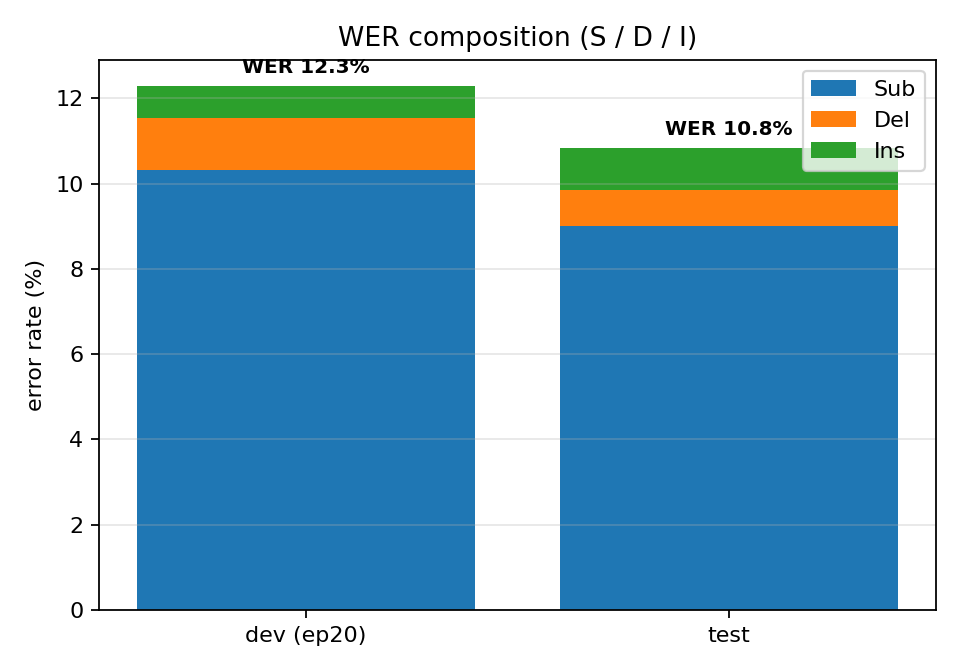
\includegraphics[width=0.6\textwidth]{res_wer_breakdown.png}
    \caption{dev 与 test 的 WER 及其 S/D/I 组成，替换错误占主导。}
    \label{fig:break}
\end{figure}

表~\ref{tab:examples} 给出若干测试样例，可见多数句子能完全识别正确，错误集中在发音相近的拼音混淆上。

\begin{table}[H]
  \centering
  \small
  \begin{tabularx}{\textwidth}{l X}
  \toprule
  类型 & 内容（拼音，加粗为差异处） \\
  \midrule
  正确 & zuo tian ta xiang cheng du shang bao ji zhe wei wei dao lai \\
  正确 & dui yu wu li ke tu de ke hu qu dao ye ba ta men qia duan le \\
  \midrule
  参考 & zhe jiang hui hen da cheng du de huan jie yang lao jin de que \textbf{kou} \\
  预测 & zhe jiang hui hen da cheng du de huan jie yang lao jin de que \textbf{kao} \\
  \midrule
  参考 & gang \textbf{mai} de ku zi bu dao shi fen zhong ni jiu nong po le \\
  预测 & gang \textbf{lai} de ku zi bu dao shi fen zhong ni jiu nong po le \\
  \midrule
  参考 & mei jun wei he hai po bu ji dai de yao dong yong \ \ di si bu bing shi \\
  预测 & mei jun wei he hai po bu ji dai de yao dong yong \textbf{you} di si bu bing shi \\
  \bottomrule
  \end{tabularx}
  \caption{测试集识别样例（参考 vs 预测）。}
  \label{tab:examples}
\end{table}

\section{进阶任务：与 AI 讨论得到的改进}
本实验的进阶改进就是第~\ref{sec:debug} 节的 \textbf{Post-LN $\rightarrow$ Pre-LN}。它既是修复也是改进：
在与 AI 讨论「为什么从零训练的 Transformer 会塌缩到全 blank」时，AI 给出的候选原因包括学习率、
特征归一化、归一化位置等；我通过控制变量的探针实验逐一验证，最终确认是\textbf{归一化位置（Post-LN vs Pre-LN）}：
Post-LN 对学习率敏感（高 LR 塌缩、低 LR 才能慢慢训），而 Pre-LN 稳健，能直接用更高的学习率更快收敛。
改进有效的根本原因在于 Pre-LN 提供了更顺畅的梯度回流路径（详见第~\ref{sec:debug} 节分析）。
此外还叠加了两个小改进：学习率的 warmup + 余弦退火、以及 Pre-LN 末尾补最终 LayerNorm，二者共同让最终
dev/test WER 进一步降低。

\section{关于 AI Coding 的思考}
\textbf{Q1（传统逐段补全 vs 全项目 Vibe Coding）}\quad
本次是一个多文件联动的完整 ASR 项目，我更多采用\textbf{基于全项目上下文的 Vibe Coding 模式}：让 AI 先梳理
「预处理$\rightarrow$模型$\rightarrow$训练$\rightarrow$推理$\rightarrow$评测」的整体框架，再在已有 \texttt{dataprocess}/\texttt{model}
接口约束下补全训练与评测。这种模式的好处是各模块接口能对齐（比如 \texttt{collate\_fn} 返回的两个长度必须原样喂给
CTC）；但纯 Vibe 也有代价——当出现「全 blank 塌缩」这类跨模块的隐性问题时，AI 很难仅凭上下文定位，仍需人来做
控制变量实验。我的体会是：\textbf{框架搭建适合 Vibe，疑难定位要回到单点、逐段验证}。

\textbf{Q2（如何定位并修正 AI 的错误代码）}\quad
关键是不把报错整段丢回给 AI「抽卡」，而是\textbf{按 ASR 的环节缩小范围、用控制变量实验逐一验证假设}。本次
loss 平坦且输出全 blank，我先用诊断脚本排除数据与长度问题；再做学习率的\textbf{双向探针}——提高 LR 仍塌缩、
但降到 $10^{-4}$ 又能训，据此意识到是 Post-LN 对学习率敏感；最终把它换成 Pre-LN，在高 LR 下稳健收敛，
锁定并解决问题。整个过程 AI 负责快速产出候选和改代码，\textbf{判断哪个假设成立、设计什么实验去验证，是我来做的}。

\textbf{Q3（与 AI 的长期共生关系与个人壁垒）}\quad
我倾向把 AI 当作「\textbf{高效的初级工程师 + 随叫随到的资料库}」：它极大降低了写样板代码、查 API、搭框架的成本，
让我把精力放在更高层的判断上。要避免被取代，我的核心壁垒是\textbf{对问题本质的理解和实验判断力}——
知道 CTC 为什么会塌缩、知道该测什么来区分假设、知道结果合不合理。AI 降低的是「写代码」的门槛，
并没有降低「看懂问题」的门槛，后者正是需要长期积累、难以被替代的能力。

\textbf{Q4（懂 ASR 与不懂 ASR 用 AI 的区别）}\quad
差别巨大。本次「全 blank 塌缩」若不懂 ASR，只会看到「训不出来」，既不知道 $100\%$ 且全删除意味着输出空串，
也想不到去比较 Post-LN/Pre-LN，只能反复让 AI 改代码碰运气，很可能困死。\textbf{懂 ASR 让我能问对问题、
判断结果是否合理、把 bug 定位到具体环节，从而精准地指挥 AI}。也就是说，领域知识决定了我是在「驾驶」AI，
还是被 AI 牵着走——这也是我在这个项目中最深的体会。

\section{结论}
本实验用 AI Coding 的方式实现了 Transformer Encoder + CTC 的中文拼音语音识别系统，主要结论如下：
\begin{enumerate}
  \item 走通了 ASR 完整流程：Fbank 提取、拼音词表、变长对齐、CTC 训练、贪心解码、WER 评测；
        实现时对齐了 blank 一致性、$[T,B,V]$ 形状、下采样后长度三个 CTC 易错点。
  \item 定位并修复了豆包模型的关键问题：Post-LN Transformer 对学习率敏感，在 $\text{lr}=10^{-3}$ 下塌缩到全 blank
        （低 $\text{lr}=10^{-4}$ 才能慢慢训）；改为 \textbf{Pre-LN + 最终 LayerNorm} 后可在高 LR 下稳健收敛，
        4 个 epoch 内 WER 即从 $100\%$ 降到 $23\%$。
  \item 最终在测试集上取得 \textbf{WER $=\testWER\%$}（dev 最优 \devWER\%），达到并优于 $30\%$ 的目标，
        错误以发音相近拼音的替换为主。
  \item 使用 AI 的核心体会是：AI 擅长搭框架、写样板、给候选，但\textbf{判断力和领域知识}决定了能否定位疑难 bug、
        判断结果是否合理——这是人相对 AI 的核心壁垒。
\end{enumerate}

\begin{thebibliography}{9}
\bibitem{ctc} A. Graves, S. Fern\'andez, F. Gomez, J. Schmidhuber.
  \emph{Connectionist Temporal Classification: Labelling Unsegmented Sequence Data with Recurrent Neural Networks}.
  ICML, 2006.
\bibitem{transformer} A. Vaswani et al. \emph{Attention Is All You Need}. NeurIPS, 2017.
  \url{https://arxiv.org/abs/1706.03762}
\bibitem{prenorm} R. Xiong et al. \emph{On Layer Normalization in the Transformer Architecture}.
  ICML, 2020. \url{https://arxiv.org/abs/2002.04745}
\end{thebibliography}

\end{document}
